\documentclass[10pt, a4paper]{report}
\usepackage[utf8]{inputenc}
\usepackage{amsfonts}
\usepackage{amsmath}
\usepackage{amssymb}
\usepackage{amsthm}
\usepackage[all,cmtip]{xy}
\usepackage{hyperref}
\usepackage[top=3cm, left=3cm,right=3cm, bottom=3cm]{geometry}
\usepackage{graphicx}
%\usepackage{subfig}
%\usepackage{subfigure}
\usepackage{caption}
\usepackage{subcaption}
\usepackage{float}
\usepackage{tikzsymbols}
\usepackage{algorithm}
\usepackage{mathtools}
\usepackage[noend]{algpseudocode}
\newcommand{\E}[0]{\mathbb{E}}
\newcommand{\Ll}[0]{\mathbb{L}}
\newcommand{\R}[0]{\mathbb{R}}
\newcommand{\Pp}[0]{\mathbb{P}}
\newcommand{\p}[0]{\mathfrak{p}}
\newcommand{\I}[0]{\mathcal{I}}
\newcommand{\F}[0]{\mathcal{F}}
\newcommand{\vv}[0]{\mathbf{v}}
\theoremstyle{definition}
\newtheorem{theorem}{Theorem}
\newtheorem{prop}{Proposition}
\newtheorem{lemma}{Lemma}
\newtheorem{coro}{Corollary}
\newtheorem{definition}{Definition}
\newtheorem*{properties*}{Properties}
\theoremstyle{remark}
\newtheorem{rmk}{Remark}
\newtheorem{ex}{Example}






\begin{document}
\begin{titlepage}
	\centering
	
\includegraphics[width=0.6\textwidth]{EPFL-Logo}\par\vspace{1cm}
	%{\scshape\LARGE École polytechnique fédérale de Lausanne \par}
	\vspace{1cm}
	{\scshape\Large Master thesis\par}
	\vspace{1.5cm}
	\hrulefill \\
	{\huge\bfseries A probabilistic approach to the classification of censored functional data \par}
	\hrulefill \\
	\vspace{2cm}
	{\Large William \textsc{Borgeaud dit Avocat}\par}
	\vfill
	{\Large
	supervised by\par
	Prof.~Victor \textsc{Panaretos}}
	
	\vfill
	
	% Bottom of the page
	{\large \today\par}
\end{titlepage}

\tableofcontents

\chapter{Introduction to Functional Data Analysis}
\section{What are functional data?}
\subsection{Explain the structure of functional data, the spaces they live in, expectation, covariance, observable discretized versions. }
\section{Statistical analysis of functional data}
\subsection{Explain the basic principles of estimation of mean and covariance with convergence rates, etc.. Also mention smoothing methods. }

\chapter{Censored functional data}
\section{Functional fragments framework}\label{introfrag}
\textit{Censored functional data} or \textit{functional fragments} are functional data that are not observed in the full domain on which they are defined. If the data live in $\Ll^2(\mathcal{I})$ for some interval $\mathcal{I} \subset \R$, an example of functional fragment is a function $f \in \Ll^2(\mathcal{J})$ for some interval $\mathcal{J}\subset \mathcal{I}$.

By the \textit{functional fragments framework}, we mean the statistical framework in which some or all of the observed data are in the form of fragments of some underlying, unobservable, functional data. In this case, the data at hand are pairs $\{(X_i,\mathcal{O}_i)\}_{i=1}^n$, where the $X_i$'s are random functions in $\Ll^2(\mathcal{O}_i)$ for some subintervals $\mathcal{O}_i$. We will often assume that the subintervals $\{\mathcal{O}_i\}_{i=1}^n$ are themselves random, in order to make the asymptotic theory more tractable. This framework often arises in practice when an observation is unavailable before or after a certain time.\\
The main issue in the functional fragments framework is to know to what extent one can recover precise information on the underlying population from the observed fragments. For example, how precisely can we estimate the mean and covariance when no curve is fully observed.\\
Following \cite{DP2}, we distinguish between two ways in which the intervals $\{\mathcal{O}_i\}_{i=1}^n$ are distributed, see Figure \ref{fig:exfrags}:\\

\noindent
\textbf{1.} A ``blanket '' regime, where the curves are typically observed on most or all of the domain. Then the number of observations at a given point of the domain is close to the total number of observations.\\
\textbf{2.} A ``banded'' regime, where the lengths of the $\mathcal{O}_i$ are bounded by some value $\delta>0$. Then, we have no explicit information on the covariance of points that are at distance larger than $\delta$.
\begin{figure}[ht]
	\centering
	\begin{subfigure}{.3\textwidth}
		\centering
		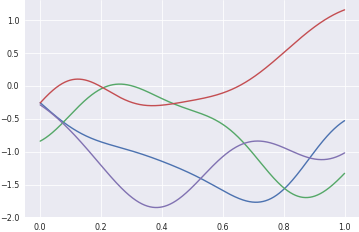
\includegraphics[width=.8\linewidth]{Code/images/21/full}
		\caption{Full curves}
	\end{subfigure}%
	\begin{subfigure}{.3\textwidth}
		\centering
		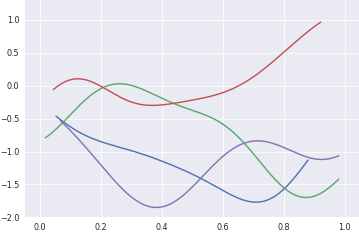
\includegraphics[width=.8\linewidth]{Code/images/21/blanket}
		\caption{\centering Fragments in the blanket regime}
	\end{subfigure}
	\begin{subfigure}{.3\textwidth}
		\centering
		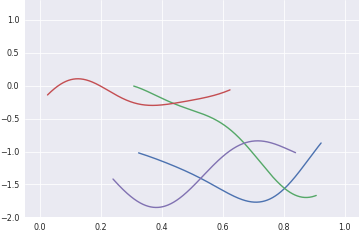
\includegraphics[width=.8\linewidth]{Code/images/21/frags}
		\caption{\centering Fragments in the banded regime}
	\end{subfigure}
	\caption{Example of functional fragments}
	\label{fig:exfrags}
\end{figure}

In the rest of this chapter, we will present various methods used in the literature dealing with those issues. 	

\section{Naive estimations}\label{naiveest}
We present here the methods presented in \cite{Kraus1}. The data are i.i.d curves $X_i$ in $\Ll^2[0,1]$ observed only on a random interval $\mathcal{O}_i \subset [0,1]$, $i=1,...,n$. To estimate the population mean $\mu = \E[X_1]$ and covariance operator $\mathcal{K} = \E[(X_1-\mu) \otimes (X_1-\mu)]$, the unobserved parts of the curves are ignored and the sample estimators are created naively as follows. The sample mean $\hat{\mu}$ is found by taking the mean of the pointwise observed values: 
\begin{equation}\label{estmufrag}
	\hat{\mu}(t) = \frac{\mathbf{1}[\exists \mathcal{O}_i \ni t ]}{\sum_{i=1}^n \mathbf{1}[t \in \mathcal{O}_i]} \sum_{i=1}^n \mathbf{1}[t \in \mathcal{O}_i] \cdot X_i(t).
\end{equation}

The covariance operator is estimated in the same fashion via its associated covariance kernel $K(\cdot,\cdot)$. The sample kernel is given by:
\begin{equation}\label{estcovfrag}
	\hat{K}(s,t) = \frac{\mathbf{1}[\exists \mathcal{O}_i \ni s,t ]}{\sum_{i=1}^n \mathbf{1}[s,t \in \mathcal{O}_i]} \sum_{i=1}^n \mathbf{1}[s,t \in \mathcal{O}_i] \cdot \left\{X_i(s)-\hat{\mu}_{st}(s)\right\}\left\{X_i(t)-\hat{\mu}_{st}(t)\right\},
\end{equation}
where  $\hat{\mu}_{st}$ is an estimation of the mean using only the curves observed at $s$ and $t$:
\[\hat{\mu}_{st}(s) = \frac{\mathbf{1}[\exists \mathcal{O}_i \ni s,t ]}{\sum_{i=1}^n \mathbf{1}[s,t \in \mathcal{O}_i]} \sum_{i=1}^n \mathbf{1}[s,t \in \mathcal{O}_i] \cdot X_i(s). \]
The sample covariance operator $\hat{\mathcal{K}}$ is then defined by 
\[\hat{\mathcal{K}}f(t) = \int_{0}^{1} \! \hat{K}(s,t)f(s) \, \mathrm{d}s.\]
We note that this operator need not be positive-definite. This can be dealt with by clipping the negative eigenvalues to zero.\\
The following proposition, proved in \cite[Prop. \!1]{Kraus1}, shows that under some assumptions on the random intervals $\{\mathcal{O}_i\}_{i=1}^n$, the above estimates enjoy the same asymptotic convergence rate as their counterparts when the curves are fully observed.
\begin{prop}
	\begin{itemize}
		\item[]
		\item[1.] Suppose that $\mathbb{E}\Vert X_1\Vert^2<\infty$ and the $\mathcal{O}_i$'s are i.i.d with $\inf_{t \in [0,1]} \Pp\left[t \in \mathcal{O}_1\right]>0$. Then 
		\[\mathbb{E}\Vert \hat{\mu}-\mu\Vert^2 = O(n^{-1}) \text{ as } n \to \infty. \]
		\item[2.] Suppose further that $\mathbb{E}\Vert X_1\Vert^4<\infty$ and that $\inf_{s,t \in [0,1]} \Pp\left[s,t \in \mathcal{O}_1\right]>0$. Then 
		\[\mathbb{E}\Vert \hat{\mathcal{K}}-\mathcal{K}\Vert^2_{HS} = O(n^{-1}) \text{ as } n \to \infty. \]
	\end{itemize}
	\qed
\end{prop}
For the covariance operator, even though the theoretical convergence rate is good, in practice the estimate is not adequate in the ``banded'' regime (see Section \ref{introfrag}). The problem is that in this regime, the estimated kernel is necessarily zero in the region $\{(s,t)\in [0,1]^2 \, \mid \, \vert s-t\vert > \delta \}$. This problem that is not present in the ``blanket'' regime, as soon as one full curve is observed, see Figure .
\begin{figure}[H]
	\centering
	\begin{subfigure}{.3\textwidth}
		\centering
		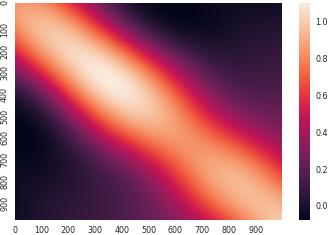
\includegraphics[width=.8\linewidth]{Code/images/22/truecov}
		\caption{Full curves}
	\end{subfigure}%
	\begin{subfigure}{.3\textwidth}
		\centering
		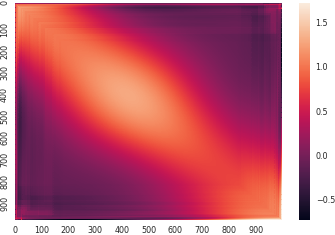
\includegraphics[width=.8\linewidth]{Code/images/22/blanketheat}
		\caption{\centering Fragments in the blanket regime}
	\end{subfigure}
	\begin{subfigure}{.3\textwidth}
		\centering
		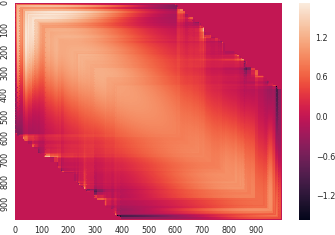
\includegraphics[width=.8\linewidth]{Code/images/22/fragsheat}
		\caption{\centering Fragments in the banded regime}
	\end{subfigure}
	\caption{Sample estimates of the covariance kernel in the different regimes}
	\label{fig:excov}
\end{figure}

\section{Curve extension}
In \cite{DH1}, the authors take the approach of manually extend the fragments by gluing some of their parts. This procedure is carried on in the context of classification, but it can readily be expended to the plain estimation of the population mean and covariance.\\
The extension of a fragment to the right is done by iteratively gluing a small section of another randomly chosen nearby fragment to the right endpoint of the original fragment. Likewise for the extension to the left. A few steps of this procedure are shown in Figure \ref{fig:gluingsteps}.
\begin{figure}[htp]
	\centering
	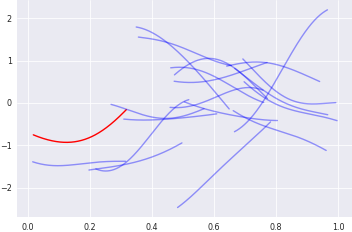
\includegraphics[width=.4\textwidth]{Code/images/23/step1}\quad
	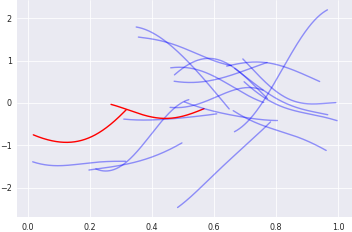
\includegraphics[width=.4\textwidth]{Code/images/23/step2}\quad
	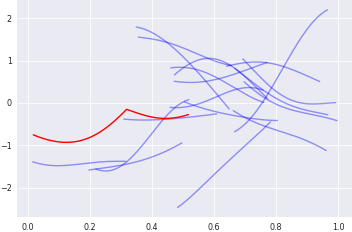
\includegraphics[width=.4\textwidth]{Code/images/23/step3}
	
	\medskip
	
	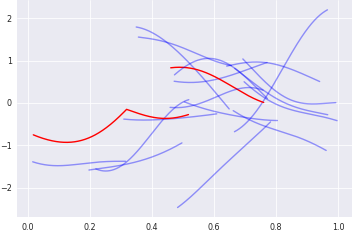
\includegraphics[width=.4\textwidth]{Code/images/23/step4}\quad
	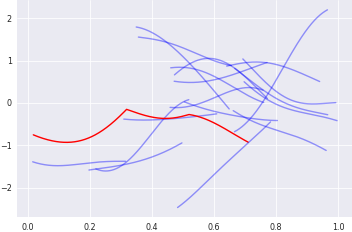
\includegraphics[width=.4\textwidth]{Code/images/23/step5}
	
	\caption{Illustration of a few steps of the gluing procedure}
	\label{fig:gluingsteps}
\end{figure}

In this way, for each fragment $(X_i, \mathcal{O}_i)$, one gets a curve $\tilde{X}_i$ defined on the entire domain. From these full curves, the sample mean and covariance can be estimated. This estimation method works both in the ``blanket'' and the ``banded'' regime, since in both cases full curves are constructed. Examples of those estimates are shown in Figure \ref{fig:gluingex}.\\
\begin{figure}[ht]
	\centering
	\begin{subfigure}{.4\textwidth}
		\centering
		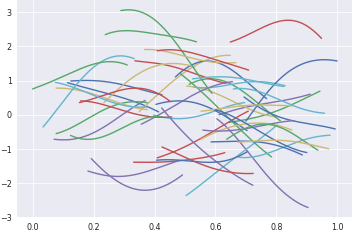
\includegraphics[width=.8\linewidth]{Code/images/23/frags}
		\caption{Fragments}
	\end{subfigure}%
	\begin{subfigure}{.4\textwidth}
		\centering
		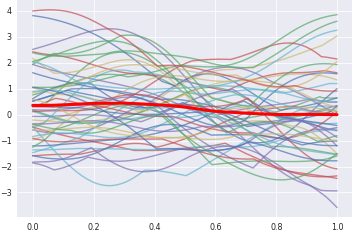
\includegraphics[width=.8\linewidth]{Code/images/23/extended}
		\caption{\centering Reconstructed curves with their mean in red}
	\end{subfigure}
	
	
	\medskip
	
	
	\begin{subfigure}{.4\textwidth}
		\centering
		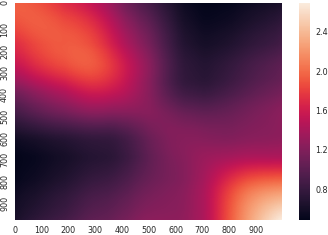
\includegraphics[width=.8\linewidth]{Code/images/23/cov}
		\caption{\centering Estimated covariance kernel form the reconstructed curves }
	\end{subfigure}
	\caption{Example of mean and covariance estimation using the gluing procedure}
	\label{fig:gluingex}
\end{figure}
To the best of our knowledge, no theoretical convergence rates for these estimates have been found. We also note that another function extension method for functional fragments is presented in \cite{DH2} by the same authors. This method assumes that discretized versions of the curves are Markov processes and then extend the fragments using this assumption.



\section{Covariance recovery}
In this section, we present the covariance recovery method of \cite{DP2}. In this paper, the authors show that under some smoothness assumptions, one can use a matrix completion method to recover the covariance matrix of a process from the observations of fragments in the ``banded'' regime. 
\subsection{Setup}\label{recovsetup}
We consider a continuous stochastic process $X \in \Ll^2[0,1]$ with mean function $\E[X]=\mu$ and covariance kernel $r(s,t) = \text{cov}\! \left\{ X(s) , X(t) \right\}$. Suppose we observe i.i.d. fragments $(X_i,\mathcal{O}_i)$ of length $\delta \in (0,1)$. Then, one can compute the estimates $\tilde{\mu}_n$ and $\tilde{r}_n$ given by Equations \ref{estmufrag} and \ref{estcovfrag}. Suppose further that we observe these fragments only on a grid of size $K$
\[ (t_1,...,t_K) \in \mathcal{T}_K = \{(x_1,...,x_K)\in \R^K \, \mid \, x_i \in I_{i,K} \}, \]
where $\{I_{i,K}\}_{i=1}^K$ is the regular partition of $[0,1]$ in intervals of length $1/K$. From these discrete observations, one can compute the mean vector $\tilde{\mu}_n^K = (\tilde{\mu}_n(t_i))_{i=1}^K$ and the covariance matrix $\tilde{R}_n^K = \{\tilde{r}_n(t_i,t_j)\}_{i,j=1}^K$. As noted above, this matrix will have a banded structure. Indeed, each fragment $X_i$ is observed only on $\mathcal{O}_i \cap \{t_i\}_{i=1}^K$, which has between $\lfloor{K\delta}\rfloor -1$ and $\lceil{K\delta}\rceil +1$ points. Thus, the matrix $\tilde{R}_n^K$ is guaranteed to have non-zero values only on the band $\{(i,j) \, \mid \, \vert i-j\vert < \lfloor{K\delta}\rfloor -1\}$. Denote by $R^K$ the true covariance matrix $\{r(t_i,t_j)\}_{i,j=1}^K$ and by $P_\delta^K \in \R^{K \times K}$ the band indicator matrix 
$$P_{\delta}^K(i,j) = \mathbf{1}\left[\, \vert i-j\vert < \lfloor{K\delta}\rfloor -1\right].$$
Then $\tilde{R}_n^K$ can realistically be seen only as an estimator of $P_{\delta}^K \circ R^K$, where ``$\circ$'' denotes the Hadamard product. \\
The question now is, under what non-parametric conditions on the process $X$ one can hope to efficiently recover the full covariance matrix $R^K$ from its banded version $P_{\delta}^K \circ R^K$? The estimation of the covariance in this setup can thus be seen as a matrix completion problem. 

\subsection{Identifiability and estimation}
The main result of \cite{DP2} is that under simple non-parametric assumptions given below, one can exactly recover the covariance matrix from its banded version. Moreover, they show that these condtions are, in some sense, necessary. These assumptions are the following:
\begin{itemize}
	\item[1.] The covariance kernel $r(s,t)$ has finite rank $q$, i.e., it admits a Mercer decomposition 
	$$r(s,t) = \sum_{j=1}^{q} \lambda_j \phi_j(s)\phi_j(t).$$
	\item[2.] The eigenfunctions $\{\phi_1,...,\phi_q\}$ are all real analytic.
\end{itemize}
The following results, shown in \cite[Prop.\! 1]{DP1}, indicate that the second condition is not as strict as it seems.

\begin{prop}
	The set of trace class covariance operators of rank at most $q$ with analytic eigenfunctions is dense in the space of rank $q$ trace class covariance operators with the nuclear norm. In particular, for any process $X  \in \Ll^2[0,1]$ with finite rank $q$ trace class operator and any $\epsilon>0$, there exists a process $Y$, satisfying the conditions above, such that 
	$$\E\Vert X-Y\Vert^2_{\Ll^2} < \epsilon.$$ \qed
\end{prop}

The main property of finite rank analytic kernel we will use is the one known as analytic continuation. We will need it in the following form, which is a special case of \cite[Corollary 1.2.6]{analprimer}:
\begin{prop}
	Let $r,l:[0,1]^2 \to \R$  be two real analytic finite rank kernels. Suppose that there exists an open set $U \subseteq [0,1]^2$ such that $r(s,t)=l(s,t)$ for all $(s,t)\in U$. Then $r(s,t)=l(s,t)$ for all $(s,t) \in [0,1]^2$, i.e., $r$ and $l$ are equal. \qed
\end{prop}
In our setup, this implies that knowing the covariance kernel on the band $\{(s,t) \in [0,1]^2 \ \mid \ \vert s-t \vert < \delta\}$ allows us to recover the kernel on the whole domain $[0,1]^2$. This shows that the model is identifiable in the sense that one can recover the true covariance from the observations of fragments. \\
In the discretized setup, this translates into the following identifiability result:
\begin{theorem}[\cite{DP2}]
	Suppose that the covariance kernel $r(s,t)$ is analytic of finite rank $q$. If $\delta$ and $K$ are such that 
	$$K>\frac{q+2}{\delta}$$
	then, for almost all $(t_1,...,t_K) \in \mathcal{T}_K$, then the covariance matrix $R^K$ is the unique solution of 
	\begin{equation}\label{matcomp}
		\min_{M \in \R{K \times K}} \text{rank}(M) \ \text{ subject to } \ \Vert P_\delta^K \circ (R^K - M) \Vert_{Frob}=0.
	\end{equation}

	Equivalently, introducing a Lagrange multiplier, for all $\tau>0$ sufficiently small,
	\[R^K = \underset{M \in R^{K\times K}}{\text{argmin}} \left\{\Vert P_\delta^K \circ (R^K - M) \Vert_{Frob}^2 + \tau \, \text{rank}(M) \right\} \]
	almost everywhere on $\mathcal{T}_K$.
	\begin{proof}
		By \cite[Theorem 4]{DP1}, all $q\times q$ minors of $R^K$ are non-zero. Moreover, the condition $K>(q+2)/\delta$ implies that $R^K$ and $P_\delta^K \circ R^K$  share at least one common $q\times q$  submatrix. Combining these two results yields that $R^K$ has rank $q$ and that $P_\delta^K \circ R^K$ has rank at least $q$. Therefore $R^K$ is a solution of the matrix completion problem \ref{matcomp}. It remains to show that it is the unique solution thereof. Let $R^*$ be another solution. Then, by design, $R^*$ has rank $q$ and is equal to $R^K$ on the band $B_\delta=\{(i,j) \, \mid \, \vert i-j\vert < \lfloor{K\delta}\rfloor -1\}$. Since $K>(q+2)/\delta$, we can find a $(q+1)\times (q+1)$ submatrix $A$ of $R^*$ with exactly one entry $x^*$ outside the band $B_\delta$, see Figure \ref{fig:matcomp}.
		\begin{figure}[ht]
		\centering
		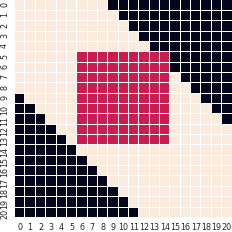
\includegraphics[width=0.5\linewidth]{Code/images/24/matcomp}
		\caption{Illustration of the matrix completion method with $K=21$, $q=8$, $\delta=0.5$. The band $B_\delta$ is colored in white and a possible $(q+1)\times (q+1)$ submatrix $A$ is colored in red.}
		\label{fig:matcomp}
		\end{figure}
		The determinant of $A$ can then be written as $ax^* + b$ where $a$ is the determinant of a $q\times q$ submatrix contained in $B_\delta$, and is thus non-zero, and $b$ depends only on the values of $R^*$ in $B_\delta$. Since $R^*$ has rank $q$, $$\det(A)=ax^*+b=0.$$ 
		Therefore, $x^*$ is uniquely determined by the values of $R^*$ in $B_\delta$, and they are themselves fixed to be equal to the values of $R^K$ in that band. Therefore, all solutions of \ref{matcomp} are equal on the entry $x^*$.\\
		One can iterate this procedure to reconstruct entirely the matrix $R^K$. The solution of \ref{matcomp} is thus unique and given by $R^K$. 
	\end{proof}
	By pluging-in the banded estimator $\tilde{R}_n$ defined in Section \ref{recovsetup}, the theorem naturally leads to the following estimator of the full matrix $R^K$:
	\begin{definition}
		Define the estimator $\hat{R}_n^K$ of $R^K$ as a minimum of 
		\begin{equation}
			\underset{0 \preceq M \in R^{K\times K}}{\text{argmin}} \left\{\Vert \tilde{R}_n^K - P_\delta^K \circ  M \Vert_{Frob}^2 + \tau_n \, \text{rank}(M) \right\},
		\end{equation}
		where $\tau_n$ is a parameter that should converge to 0 as $n$ goes to infinity. From this estimator of the covariance matrix, one can estimate the covariance kernel by the step function
		\begin{equation}
			\hat{r}_n(s,t) = \hat{R}_n^K(i,j) \ \text{ if } \ (s,t)\in I_{i,K}\times I_{j,K}.
		\end{equation}
		\qed
	\end{definition}
\end{theorem}
We have the following consistency result.
\begin{theorem}
	Assume $\E\Vert X_i \Vert^4_{\Ll^2} < \infty$, the intervals $\{\mathcal{O}_1,...,\mathcal{O}_n\}$ are i.i.d. independent of the $X_i$'s and that $\inf_{s,t \in [0,1]} \Pp\left[s,t \in \mathcal{O}_1\right]>0$. Let $K^*= \lfloor (q+2)/\delta\rfloor + 1$ be the critical resolution. Then, if $\tau_n \to 0$, for almost any grid in $\mathcal{T}_K$, 
	\begin{equation}
		\int\int_{[0,1]^2}  \left(\hat{r}_n^K(x,y)-r(x,y)\right)^2 dxdy \leq O_{\Pp}(1/n) + 4K^{-2} \sup_{x,y \in [0,1]} \Vert \nabla r(x,y)\Vert_2^2,
	\end{equation}
	uniformly in $K$, for any refinement $K=m\times K^*$.\qed
\end{theorem}

\subsection{Numerical implementation}
The implementation of the estimator $R^K_n$ is explained in detail in \cite[Section 5]{DP2}. Roughly, it consists of two steps:
\begin{itemize}
	\item[1.] Find an approximate minimum $M_i$ of 
	$$\min_{0\preceq M \in \R^{K\times K}} \Vert \tilde{R}_n^K - P_{\delta}^K \circ M||^2_{Frob} \text{ subject to rank}(M)\leq i $$ 
	for $i \in \{1,...,\lceil K\delta\rceil-3 \}$. This can be done by writing $M_i = \gamma \gamma^T$ with $\gamma \in \R^{K\times i}$ and optimizing on $\gamma$ using general purpose optimization algorithm, e.g., BFGS. Note that the objective function is not convex in $\gamma$. However, numerical experiments indicate that local minima are good enough.
	\item[2.] Compute the objective value $f(i)$ of $M_i$ for all $i \in \{1,...,\lceil K\delta\rceil-3 \}$ and take $\hat{R}_n^K = M_j$ for the rank $j$ after which the function $f$ does not decrease much more.
\end{itemize}

\subsection{Example}
We present here a numerical example of the covariance recovery method. Let $r'(s,t)=\min(s,t)$ be the covariance kernel of the brownian motion and $r(s,t)$ be its projection on its first 10 eigenfunctions. Then $r(s,t)$ is a rank $10$ analytic kernel. We take $\mu \equiv 0$, $n=100$, $K=50$, $\delta=0.6$ in the following. Example of fragments along with the estimated mean $\tilde{\mu}_n^K$ are shown in Figure \ref{fig:fragex}.
\begin{figure}
\centering
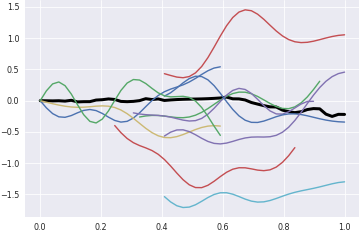
\includegraphics[width=0.7\linewidth]{Code/images/24/fragex}
\caption{Plot of 10 fragments (out of the total 100), and the estimated mean in black. }
\label{fig:fragex}
\end{figure}
The true covariance matrix $R^K$ along with the banded estimator $\tilde{R}_n^K$ are shown in Figure \ref{fig:truetrunccov}.
\begin{figure}[H]
	\centering
	\begin{subfigure}{.5\textwidth}
		\centering
		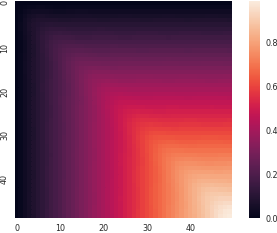
\includegraphics[width=.8\linewidth]{Code/images/24/truecov}
		\caption{True covariance matrix}
	\end{subfigure}%
	\begin{subfigure}{.5\textwidth}
		\centering
		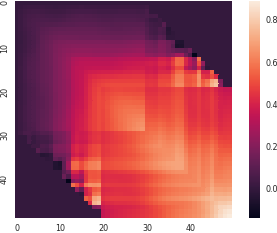
\includegraphics[width=.8\linewidth]{Code/images/24/trunccov}
		\caption{Banded estimator}
	\end{subfigure}
	\caption{}
	\label{fig:truetrunccov}
\end{figure}
The relative error $\Vert R^K - \tilde{R}_n^K\Vert / \Vert R^K \Vert$ is 27.2\% here. We now perform the first step of the implementation, as described in the previous section. A plot of the objective values for $i \in \{1,...,10\}$ is shown in Figure \ref{fig:obvals}.
\begin{figure}
\centering
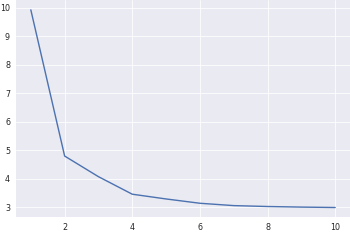
\includegraphics[width=0.7\linewidth]{Code/images/24/obvals}
\caption{Objective value in function of the rank.}
\label{fig:obvals}
\end{figure}
From this plot, we decide to choose the rank of the estimator to be $i=5$. The resulting estimator $\hat{R}_n^K = M_5$  is shown in Figure \ref{fig:estcov}.
\begin{figure}
\centering
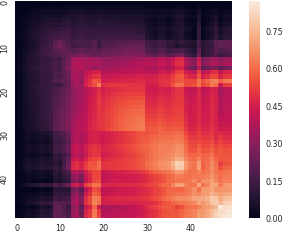
\includegraphics[width=0.7\linewidth]{Code/images/24/estcov}
\caption{Estimated covariance matrix $\hat{R}_n^K$.}
\label{fig:estcov}
\end{figure}
The relative error with this estimate is $\Vert R^K - \hat{R}_n^K\Vert / \Vert R^K \Vert = 21.3\%$. By using the matrix completion method, we have thus achieved a gain of 28\% in relative error compared to the naive estimator $\tilde{R}_n^K$ described in Section \ref{naiveest}.


\chapter{Gaussian measures in Hilbert space}
\section{Gaussian measures in finite dimensions}
Before exploring the construction and properties of infinite dimensional Gaussian measures, we start by going through the basic definitions and properties of finite dimensional Gaussian measures in ways that are easily generalizable to the infinite dimensional case.\\
We start with one-dimensional Hilbert spaces, i.e., the real line.
\begin{definition}
	Let $a\in \R$ and $\sigma^2>0$  be parameters. A measure $\mu$ on the Borel $\sigma$-algebra $\mathcal{B}(\R)$ is said to be a \emph{Gaussian measure} with mean $a$ and variance $\sigma^2$ if 
	\begin{equation}
		\mu(A) = \int_{A} \frac{1}{\sqrt{2\pi\sigma^2}}e^{-\frac{(x-a)^2}{2}}dx, \ \ \forall A \in \mathcal{B}(\R),
	\end{equation}
	where the integral is with respect to the Lebesgue measure on $\R$. We denote this measure $N_{a,\sigma^2}$. \qed
\end{definition}
We have the following elementary properties:
\begin{properties*}
	\begin{itemize}
		\item[]
		\item[1.] The measure $N_{a,\sigma^2}$ indeed has mean $a$ and variance $\sigma^2$, i.e., 
		\[ \int_{\R}x N_{a,\sigma^2}(dx) = a \ \text{ and } \ \int_{\R}(x-a)^2 N_{a,\sigma^2}(dx)=\sigma^2. \]
		\item[2.] The measure $N_{a,\sigma^2}$ is equivalent to the Lebesgue measure $\lambda$ on $\mathcal{B}(\R)$, and its Radon-Nykodim derivative is given by 
		\[\frac{dN_{a,\sigma^2}}{d\lambda}(x) = \frac{1}{\sqrt{2\pi\sigma^2}}e^{-\frac{1}{2}(x-a)^2}. \]
		\item[3.] The Fourier transform of $N_{a,\sigma^2}$ is 
		\[\widehat{N_{a,\sigma^2}}(y) = \int_{\R} e^{iyx} N_{a,\sigma^2}(dx) = e^{iay-\frac{1}{2}\sigma^2 y^2} \]
		\item[4.] If $X$ is a random variable with distribution $N_{a,\sigma^2}$ and $\alpha,\beta \in \R$, then $\alpha X + \beta$ has distribution $N_{\alpha a + \beta, \alpha^2 \sigma^2}$. 
	\end{itemize}\qed
\end{properties*}
Note that one can also consider the limiting case $\sigma^2 = 0$, in which case the measure $N_{a,0}$ is the Dirac measure concentrated in $a$. \\
The definition of a Gaussian measure in arbitrary finite dimension relies on the following intuition. We would like these measures to ``look like'' one-dimensional Gaussian measure in every direction. Formally, this translates to:
\begin{definition}
	For $f \in \R^d$, let $f^*$ denote the linear functional $f^*(x)=\langle f,x\rangle$. A measure $\mu$ on $\R^d$ is said \emph{Gaussian} if for all $f \in \R^d$, the pushforward  measure $f^*_{\sharp}\mu$ on $\R$ is Gaussian.\qed
\end{definition}
For $\mu$ and $f$ as above, call $x_f$ the mean of $f^*_{\sharp}\mu$. Since the mean is linear, the function $f\mapsto x_f$ is linear, and thus, there exists some $a \in \R^d$  with $x_f = \langle a,f\rangle$. Then, 
$$\int_{\R^d} x \mu(dx) =  a.$$
Now, consider the function
$$\R^d \times \R^d \ni (f,g) \mapsto \beta(f,g) = \int_{\R^d} \langle f,x-a\rangle \langle g,x-a\rangle \mu(dx) \in \R. $$
It is easy to see that this gives a symmetric positive semidefinite bilinear form on $\R^d$ and thus has a representation $\beta(f,g)=\langle Qf,g\rangle$ for some p.s.d. matrix $Q$. Moreover, $\beta(f,f)=\langle Qf,f\rangle$ is the variance of $f^*_{\sharp}\mu$. \\
Finally, we note that the measure is uniquely determined by these two parameters $a\in \R^d$ and $Q \in \R^{d \times d}_{\succeq 0}$, since the Fourier transform of $\mu$ depends solely on them:
\begin{equation}\label{charcgau}
	\widehat{\mu}(f) = \int_{\R^d}e^{i\langle f,x\rangle}\mu(dx) = \int_{\R} e^{iy} f^*_{\sharp}\mu(dy) = e^{i\langle f,a\rangle - \frac{1}{2} \langle Qf,f\rangle }.
\end{equation}
Finally, we prove that this correspondence between Gaussian measure on $\R^d$ and pairs $(a,Q)$ is bijective. 
\begin{prop}\label{uniquegaussfin}
	For any $a \in \R^d$ and any p.s.d. matrix $Q \in \R^{d \times d}_{\succeq 0}$, there exists a unique Gaussian measure $\mu$ on $\R^d$ having Fourier transform given by Equation \ref{charcgau}. This measure is denoted $N_{a,Q}$.
	\begin{proof}
		The uniqueness is immediate. For the existence, consider the measure $\nu$ on $\mathcal{B}(\R^d)$ given by the product measure $$\nu = \bigtimes_{i=1}^d N_{0,1}.$$ Let $L:\R^d \to \R^d$ be defined by $L(x)= a + Q^{1/2} x$ and define $\mu$ as $L_{\sharp}\nu$. Then,
		$$\widehat{\mu}(f) = \int_{\R^d}e^{i\langle f,x\rangle}\mu(dx) = \int_{\R^d} e^{i\langle f,a+Q^{1/2}y\rangle} \nu(dy) = e^{i\langle f,a\rangle} \int_{\R^d} e^{i\langle Q^{1/2}f,y\rangle} \nu(dy) = e^{i\langle f,a\rangle - \frac{1}{2} \langle Qf,f\rangle },$$
		where the last equality is given by Fubini's theorem and $\widehat{N_{0,1}}(t)= e^{-\frac{1}{2}t^2}$.	
	\end{proof}
\end{prop} 
We have the following properties:
\begin{properties*}
	\begin{itemize}
		\item[]
		\item[1.] The measure $N_{a,Q}$ indeed has covariance matrix $Q$, i.e., if $X\sim N_{a,Q}$
		\[ Q_{ij} = cov\left(X_i,X_j\right). \]
		\item[2.] The support of $N_{a,Q}$ is the image of $Q$.
		\item[3.] If $Q$ is non-singular, the measure $N_{a,Q}$ is equivalent to the Lebesgue measure $\lambda^n$ on $\mathcal{B}(\R^n)$, and its Radon-Nykodim derivative is given by 
		\[\frac{dN_{a,Q}}{d\lambda^n}(x) = \frac{1}{\sqrt{\vert 2\pi Q \vert }}e^{-\frac{1}{2}(x-a)^T Q^{-1} (x-a)}. \]
		\item[4.] If $X$ is a random variable with distribution $N_{a,Q}$ and $\beta \in \R^m$, $A \in \R^{m\times n}$, then $A X + \beta$ has distribution $N_{A a + \beta, AQA^T}$. 
	\end{itemize}\qed
\end{properties*}

\section{Gaussian measures in infinite dimensions}
We now investigate the construction and properties of Gaussian measures in infinite dimensional space, with a focus on separable Hilbert spaces. Our exposition follows those of \cite{prato1} and \cite{prato2}.\\
The following results demonstrates the main reason why measure theory is much more complicated in infinite dimension: there is no equivalent of the Lebesgue measure in any infinite dimensional normed vector space.
\begin{prop}
	Let $(V,\Vert \cdot \Vert)$ be an infinite dimensional separable normed vector space. If $\mu$ is a measure on $V$ that is locally finite and translation invariant, then $\mu(A) \equiv 0$. 
	\begin{proof}
		Suppose such a measure $\mu$ exists. Let $B$ be an open ball with finite measure. By Riesz's lemma, $B$ contains the countable disjoint union of open balls $\{B_n\}_{n=1}^\infty$ each with same radius $\delta$. Since $\mu$ is translation invariant, these balls all have the same measure. Then we get the following inequality
		$$\mu\left(\sqcup_{n=1}^\infty B_n\right) = \sum_{n=1}^{\infty}\mu(B_n) = \sum_{n=1}^{\infty}\mu(B_1) \leq \mu(B) < \infty.$$
		Thus, $\mu(B_1)=0$ and the same holds for all open balls of radius $\delta$. Since $V$ is separable, it can be covered by a countable union of such open balls. Thus $\mu(V)=0$.
	\end{proof}
\end{prop}
Thus, in contrast with the finite dimensional case, there is no standard measure with respect to which one can define Radon-Nikodym densities. In some sense, this explains why most multivariate statistics tool do not apply in functional data analysis. The reason is that the concept of likelihood is ill-defined in infinite dimensions.\\
Luckily, our definition of multivariate Gaussian measures does not depend on densities with respect to the Lebesgue measure. It can therefore be generalized easily.
\begin{definition}
	Let $(E,\Vert \cdot \Vert)$ be a Banach space. A measure $\mu$ on $\mathcal{B}(E)$ is said \emph{Gaussian} if for all $f \in E^*$, the pushforward measure $f_\sharp \mu$ is Gaussian on $\mathcal{B}(\R)$. \qed
\end{definition}
For Hilbert spaces, the dual space is isomorphic to the original space. Thus the definition simplifies to:
\begin{definition}
	For $f \in H$, let $f^*$ denote the linear functional $f^*(x)=\langle f,x\rangle$. A measure $\mu$ on $H$ is said \emph{Gaussian} if for all $f \in H$, the pushforward  measure $f^*_{\sharp}\mu$ on $\R$ is Gaussian.\qed
\end{definition}
This last definition is exactly the same as that for Gaussian measure in finite dimensions. We will thus use the same strategy as in the finite dimensional case to find parameters characterizing a given measure. We will need the following technical lemma, given in \cite[Lemma 2.15]{prato2}.
\begin{lemma}
	Let $\mu$ be a probability measure on a separable Hilbert space $H$, such that there exists $k\in \mathbb{N}$ with
	$$\int_H \vert \langle h,x\rangle\vert^k \mu(dx) < \infty, \ \ \forall h \in H.$$
	Then, there exists some constant $c>0$ such that for all $h_1,h_2,...,h_k \in H$, 
	$$\left\vert\int_H \langle h_1,x\rangle\langle h_2,x\rangle...\langle h_k,x\rangle   \mu(dx) \right\vert \leq c\Vert h_1\Vert\Vert h_2\Vert...\Vert h_k\Vert.$$
	\begin{proof}
		Consider the family of closed sets 
		$$U_n = \{h\in H \, \mid \, \int_H \vert \langle h,x\rangle\vert^k \mu(dx) \leq n \}, \ n \in \mathbb{N}.$$
		By assumtion, the union of the $U_n$ is all of $H$. By Baire's category theorem, this implies that one of them, say $U_{n_0}$ has non-empty interior. This implies that for some $z \in U_{n_0}$ and some $r > 0$, the open ball $B(z,r)$ is contained in $U_{n_0}$. In other words, for all $y\in H$ with $\Vert y \Vert < r$, it holds that
		$$ \int_H \vert \langle z+y,x\rangle\vert^k \mu(dx) \leq n_0.$$
		Now, using the general inequality (provable using Holder's inequality)
		$$\vert a-b\vert^k \leq 2^k \vert a\vert^k + 2^k \vert b \vert^k, \ a,b \in \R,$$
		we get
		$$\int_H \vert \langle y,x\rangle\vert^k \mu(dx) \leq 2^k\int_H \vert \langle z+y,x\rangle\vert^k \mu(dx) + 2^k\int_H \vert \langle z,x\rangle\vert^k \mu(dx) \leq 2^{k+1}n_0.$$
		For all $z \in H$, $\frac{r}{2\Vert z \Vert}z$ has norm less than $r$. Therefore, for all $z\in H$, 
		$$\int_H \vert \langle z,x\rangle\vert^k \mu(dx) \leq 2^{2k+1}r^{-k}n_0\Vert z \Vert^k \coloneqq c\Vert z \Vert^k.$$
		Finally, using Holder's inequality, we get
		\begin{eqnarray*}
			\left\vert\int_H \langle h_1,x\rangle\langle h_2,x\rangle...\langle h_k,x\rangle   \mu(dx) \right\vert & \leq & \int_H\left\vert \langle h_1,x\rangle\langle h_2,x\rangle...\langle h_k,x\rangle \right\vert  \mu(dx) \\ 
			& \leq & \left(\int_H\left\vert \langle h_1,x\rangle\right\vert^k \mu(dx)\right)^{1/k} ... \left(\int_H\left\vert \langle h_k,x\rangle\right\vert^k \mu(dx)\right)^{1/k} \\
			& \leq & c\Vert h_1\Vert\Vert h_2\Vert...\Vert h_k\Vert.
		\end{eqnarray*}
	\end{proof}
\end{lemma} 

Now consider the linear functional
$$ H \ni f \mapsto \alpha(f)=\int_{H}\langle f,x\rangle \mu(dx) \in \R.$$
By the previous lemma, it is continuous. Thus, by Riesz's representation theorem, there exists some $a \in H$ with $\alpha(f)=\langle f,a\rangle$ for all $f\in H$. We call $a$ the \emph{mean} of $\mu$. Next, consider the symmetric bilinear form 
$$H \times H \ni (f,g) \mapsto \beta(f,g) = \int_{H} \langle f,x-a\rangle \langle g,x-a\rangle \mu(dx) \in \R.$$
By the lemma, it is bounded. Therefore, by Riesz's representation theorem for bilinear forms (see e.g. \cite[Theorem 4.3.13]{hilb}), there exists a bounded self-adjoint operator $Q$ on $H$ such that $\beta(f,g) = \langle Qf,g\rangle$ for all $	f,g\in H$. We call $Q$ the \emph{covariance operator} of $\mu$. From 
$$\langle Qf,f\rangle = \int_{H} \langle f,x-a\rangle^2 \mu(dx) \geq 0,$$
we also get that $Q$ is non-negative. If $Q$ were compact, one could use the nice spectral theory of self-adjoint compact operators to study $Q$. In fact, the following stronger results holds:
\begin{theorem}
	The operator $Q$ defined above is trace class.
	\begin{proof}
		See \cite[Prop.\! 2.16]{prato2}
	\end{proof}
\end{theorem}
\begin{coro}
	The operator $Q$ is Hilbert-Schmidt and compact.\qed
\end{coro}
Moreover, one can show that 
$$\mathrm{Tr}(Q) = \int_H \Vert x-a\Vert^2 \mu(dx).$$
This is analogous to the result in finite dimensions that the trace of the covariance matrix is equal to the total variance of the measure.\\
The Fourier transform of $\mu$ can easily be found using the results above:
$$\widehat{\mu}(f) = e^{i\langle h,a\rangle - \frac{1}{2} \langle Qf,f\rangle }.$$
We will need the following result, proved in \cite[Prop.\! 2.5]{prato2}
\begin{prop}
	Let $H$ be a separable Hilbert space and $\mu, \nu$ be probability measures on $\mathcal{B}(H)$. If the Fourier transform $\hat{\mu},\hat{\nu}$ are equal on $H$, then $\mu = \nu$ on $\mathcal{B}(H)$.
\end{prop}
We are now ready to prove the analogue of Proposition \ref{uniquegaussfin} in infinite dimensions.
\begin{theorem}\label{uniquegausshilb}
	Let $a$ be an element of $H$ and $Q$ a non-negative trace class operator on $H$. Then, there exists a unique Gaussian measure with mean $a$ and covariance operator $Q$.
	\begin{proof}
		Uniqueness follows from the previous proposition. For the existence, let $\{\lambda_i, \phi_i \}_{i=1}^\infty$ be a complete orthogonal system of eigenvectors of $Q$, i.e., $\{\phi_i\}_{i=1}^\infty$ forms a complete orthonormal basis of $H$ and 
		$$Q = \sum_{i=1}^{\infty} \lambda_i\ \phi_i \otimes \phi_i.$$
		Let ${\xi_i}_{i=1}^\infty$ be a sequence of i.i.d. standard Gaussian random variables in $\R$ defined on a probability space $(\Omega,\mathcal{F},\Pp)$. Let $X$ be the random element of $H$ defined by 
		$$X = a + \sum_{i=1}^{\infty} \sqrt{\lambda_i} \xi_i \phi_i.$$
		The sum converges in $\Ll^2(\Omega,H)$ since $\mathrm{Tr}(Q) = \sum_{i=1}^{\infty}\lambda_i<\infty$ and
		$$\E\Vert \sum_{i=m}^{\infty} \sqrt{\lambda_i} \xi_i \phi_i \Vert^2 = \E\left[\sum_{i=m}^{\infty} \lambda_i \xi_i^2 \right] = \sum_{i=m}^{\infty}\lambda_i \stackrel{m\to \infty}{\longrightarrow} 0.$$
		Thus $X$ is a well defined element of $\Ll^2(\Omega,H)$. Let $\mu$ be its associated measure on $H$. Its Fourier transform is given by 
		\begin{eqnarray}
			\widehat{\mu}(f) & = & \int_H e^{i \langle f,h\rangle} \mu(dh)\\
			& = & \int_{\Omega} e^{i \langle f,X\rangle} \Pp(dX)\\ 
			& = & \int_{\Omega} e^{i \langle f,a\rangle + i\sum_{i=1}^{\infty}\sqrt{\lambda_i}\xi_i\langle f,\phi_i\rangle} \Pp(dX)\\
			& = & e^{i\langle f,a \rangle}\prod_{i=1}^{\infty} \int_{\Omega} e^{i\sqrt{\lambda_i}\langle f,\phi_i\rangle\xi_i} \Pp(dX)\\
			& = & e^{i\langle f,a \rangle - \frac{1}{2} \sum_{i=1}^{\infty} \lambda_i \langle f,\phi_i\rangle^2} = e^{i\langle f,a \rangle - \frac{1}{2}\langle Qf,f\rangle}
		\end{eqnarray}
		Therefore, the law of $X$ is Gaussian with mean $a$ and covariance operator $Q$.
	\end{proof}
\end{theorem}
We denote by $N_{a,Q}$ this measure. It has the following property.
\begin{prop}\label{lingausshilb}
	Let $H,K$ be separable Hilbert spaces and $B:H\to K$ a continuous linear map. Let $N_{a,Q}$ be a Gaussian measure on $H$. Then, the induced measure on $K$ is Gaussian with
	$$B_\sharp N_{a,Q} = N_{Ba, BQB^*},$$
	where $B^*:K \to H$ is the adjoint of $B$. 
	\begin{proof}
		For any $k\in K$, we have 
		\begin{eqnarray}
			\widehat{B_\sharp N_{a,Q}}(k) & = & \int_K e^{i\langle k,y\rangle} B_\sharp N_{a,Q}(dy)=\int_H e^{i\langle k,Bx\rangle} N_{a,Q}(dx)\\
			 &= & \int_H e^{i\langle B^*k,x\rangle} N_{a,Q}(dx) = \widehat{N_{a,Q}}(B^*k)\\
			 & = & e^{i\langle B^*k,a\rangle -\frac{1}{2}\langle QB^*k,B^*k\rangle} = e^{i\langle k,Ba\rangle -\frac{1}{2}\langle BQB^*k,k\rangle}
		\end{eqnarray}
	\end{proof} 
\end{prop}

\section{The Feldman-Hajek theorem}
Let $N_{a_1,Q_1}$ and $N_{a_2,Q_2}$ be Gaussian measures. We want to investigate the conditions one can impose on $a_i, Q_i$, $i=1,2$, that make the two measures either singular or equivalent.\\ 
We recall that two measures $\mu,\nu$ on $(\Omega,\mathcal{F})$ are said \emph{singular} if there exists disjoint sets $A,B\in \mathcal{F}$ whose union is $\Omega$, with $\mu(B)=\nu(A)=0$. We say that $\mu$ is absolutely continuous with respect to $\nu$, denoted $\mu << \nu$ if 
$$\forall A \in \mathcal{F}, \ \ \nu(A) = 0 \implies \mu(A)=0.$$ 
Finally, we say that $\mu$ and $\nu$ are equivalent if we have both $\mu << \nu$ and $\nu << \mu$.\\
In finite dimensions, the problem is easy. Let $N_{a_1,Q_1}$ and $N_{a_2,Q_2}$ be Gaussian measures on $\R^d$, then
\begin{itemize}
	\item[\textbf{Case 1}] If $Q_1$ and $Q_2$ have the same range and $a_2-a_1$ belongs to this range, then $N_{a_1,Q_1}$ and $N_{a_2,Q_2}$ are equivalent.
	\item[\textbf{Case 2}] Otherwise, they are singular.
\end{itemize}
It is a remarkable result that roughly the same conclusion holds in infinite dimensions. Indeed, we will show next that two Gaussian measures on a separable Hilbert space are either equivalent or singular. Moreover, the conditions for them to be equivalent are quite restrictive, as opposed to the finite-dimensional case, where it suffices for the covariance matrices to be non-singular.\\
First, we need to study the notion of \emph{Hellinger integral} and \emph{Hellinger distance}. The latter defines a distance on probability measures giving information on their mutual singularity.
\begin{definition}
	Let $\mu,\nu$ be probability densities on $(\Omega,\mathcal{F})$. The \emph{Hellinger integral} $H(\mu,\nu)$ is defined by
	$$H(\mu,\nu) = \int_{\Omega} \sqrt{\frac{d\mu}{d\lambda}\frac{d\nu}{d\lambda}}\ d\lambda,$$
	where $\lambda$ is some probability measure on $(\Omega,\mathcal{F})$ with respect to which both $\mu$ and $\nu$ are absolutely continuous. The \emph{Hellinger distance} $d(\mu,\nu)$ is defined by 
	$$d^2(\mu,\nu) = 1-H(\mu,\nu)= \frac{1}{2}\int_\Omega \left(\sqrt{\frac{d\mu}{d\lambda}}-\sqrt{\frac{d\nu}{d\lambda}}\right)^2 d\lambda. $$
\end{definition}  
We have the following properties:
\begin{properties*}
	\begin{itemize}
		\item[] 
		\item[1.] A probability measure $\lambda$ with $\mu,\nu << \lambda$ always exists.
		\item[2.] The definitions do not depend on the measure $\lambda$. 
		\item[3.] For any $\mu,\nu$, the Hellinger integral, and thus the Hellinger distance, are bounded between $0$ and $1$.
		\item[4.] The measures $\mu$ and $\nu$ are singular if and only if $H(\mu,\nu)=0$. 
		
	\end{itemize}
	\begin{proof}
		\begin{itemize}
			\item[1.] Take $\lambda = \frac{1}{2}(\mu + \nu)$.
			\item[2.] Let $\lambda'$ be another measure with $\mu,\nu << \lambda'$. Then,
			$$\mu,\nu << \lambda,\lambda' << \chi \coloneqq \frac{1}{2}(\lambda+\lambda')$$
			and 
			$$\int_{\Omega} \sqrt{\frac{d\mu}{d\lambda}\frac{d\nu}{d\lambda}}\ d\lambda = \int_{\Omega} \sqrt{\frac{d\mu}{d\lambda}\frac{d\nu}{d\lambda}}\ \frac{d\lambda}{d\chi} d\chi = \int_{\Omega} \sqrt{\frac{d\mu}{d\lambda}\frac{d\lambda}{d\chi}\frac{d\nu}{d\lambda}\frac{d\lambda}{d\chi}}\  d\chi = \int_{\Omega} \sqrt{\frac{d\mu}{d\chi}\frac{d\nu}{d\chi}}\ d\chi$$
			and the same chain of equalities holds with $\lambda'$. Thus,
			$$\int_{\Omega} \sqrt{\frac{d\mu}{d\lambda}\frac{d\nu}{d\lambda}}\ d\lambda = \int_{\Omega} \sqrt{\frac{d\mu}{d\chi}\frac{d\nu}{d\chi}}\ d\chi = \int_{\Omega} \sqrt{\frac{d\mu}{d\lambda'}\frac{d\nu}{d\lambda'}}\ d\lambda'.$$
			\item[3.] Using the Cauchy-Schwartz inequality, this follows from 
			$$0 \leq H(\mu,\nu) = \int_{\Omega} \sqrt{\frac{d\mu}{d\lambda}\frac{d\nu}{d\lambda}}\ d\lambda \leq \left(\int_{\Omega} \frac{d\mu}{d\lambda}d\lambda\right)^{1/2} \left(\int_{\Omega} \frac{d\nu}{d\lambda}d\lambda\right)^{1/2} = 1.$$
			\item[4.] Suppose $\mu \bot \nu$. Then, there exists disjoint sets $A,B \in \mathcal{F}$ such that $\Omega=A\cup B$ with $\mu(A)=1=\nu(B)$. Then
			$$H(\mu,\nu) = \int_{A} \sqrt{\frac{d\mu}{d\lambda}\frac{d\nu}{d\lambda}}\ d\lambda + \int_{B} \sqrt{\frac{d\mu}{d\lambda}\frac{d\nu}{d\lambda}}\ d\lambda = 0.$$
			Conversely, suppose $H(\mu,\nu)=0$ and let $f=\frac{d\mu}{d\lambda},g=\frac{d\nu}{d\lambda}$. Then, we have 
			$$\int_{\Omega} \sqrt{fg} \ d\lambda = 0.$$
			Therefore, $\lambda\left(\{fg=0\}\right)=1$, and since $\mu,\nu << \lambda$, it follows that 
			$$\mu\left(\{fg=0\}\right)=1=\nu\left(\{fg=0\}\right).$$
			Now, let $A=\{g=0\}$,$B = \{f=0\}$ and $C = \{fg=0\}$ so that $\mu(B)=\int_B f d\lambda=0$ and $\nu(A)=\int_A g d\lambda=0$. Since $C = A \cup B$, defining $\tilde{A} = (C\backslash B) \sqcup (\Omega\backslash C)$ yields $\Omega= \tilde{A} \sqcup B$ and 
			$$\mu(\tilde{A}) = \mu(C) - \mu(B) + (1-\mu(C)) = 1 \ \text{ and } \ \nu(B) = \nu(C) - \nu(A \backslash B) = 1.$$ 
			Thereby, $\mu$ and $\nu$ are singular.
		\end{itemize}
	\end{proof}
\end{properties*}
The reason we want to study the Hellinger integral in the context of measures on Hilbert spaces is that it behaves well with respect to infinite products. Let us start with finite products.
\begin{prop}
	Let $\mu_1,\mu_2,\nu_1,\nu_2$ be probability measures on $(\Omega,\mathcal{F})$. Consider the product measures $\mu_1\times \mu_2$ and $\nu_1\times \nu_2$ on the product space $(\Omega \times \Omega, \mathcal{F}\otimes \mathcal{F})$. Then, 
	$$H(\mu_1\times \mu_2,\nu_1\times \nu_2) = H(\mu_1,\nu_1)H(\mu_2,\nu_2).$$
	\begin{proof}
		Let $\lambda_1,\lambda_2$ be measures such that $\mu_1,\nu_1 <<\lambda_1$, and  $\mu_2,\nu_2 <<\lambda_2$. Then, for $A_1,A_2 \in \mathcal{F}$,
		\begin{eqnarray*}
			(\lambda_1 \times\lambda_2)\left(A_1 \times A_2\right) =  \lambda_1(A_1)\lambda_2(A_2) = 0 & \implies & \mu_1(A_1)\mu_2(A_2) = 0 \text{ and } \nu_1(A_1)\nu_2(A_2) = 0  \\
			& \implies & (\mu_1\times \mu_2)(A_1 \times A_2),(\nu_1\times \nu_2)(A_1 \times A_2)=0.
		\end{eqnarray*}
	Since rectangular sets like $A_1 \times A_2$ generate $\mathcal{F}\otimes \mathcal{F}$, we get that 
	$(\mu_1\times \mu_2),(\nu_1\times \nu_2) << (\lambda_1\times \lambda_2)$.
	Now, define $f_i = \frac{d\mu_i}{d\lambda_i}$, $g_i = \frac{d\nu_i}{d\lambda_i}$. Then, by Fubini's theorem,
	$$\int_{A_1\times A_2} d(\mu_1 \times \mu_2) = \int_{A_1} d\mu_1\int_{A_2}d\mu_2 =  \int_{A_1} f_1 d\lambda_1\int_{A_2}d\lambda_2 = \int_{A_1\times A_2} f_1f_2 d(\lambda_1 \times \lambda_2).$$
	Thus, $f_1f_2 = \frac{d(\mu_1 \times \mu_2)}{d(\lambda_1 \times \lambda_2)}$ and similarly, $g_1g_2 = \frac{d(\nu_1 \times \nu_2)}{d(\lambda_1 \times \lambda_2)}$. Finally, we conclude with
	$$H(\mu_1\times \mu_2,\nu_1\times \nu_2) = \int_{\Omega \times \Omega} \sqrt{f_1f_2g_1g_2}d(\lambda_1\times \lambda_2) = \int_{\Omega} \sqrt{f_1g_1}d\lambda_1\int_{\Omega} \sqrt{f_2g_2}d\lambda_2 = H(\mu_1,\nu_1)H(\mu_2,\nu_2).$$	
	\end{proof}
\end{prop}

\begin{coro}
	Let $\{\mu_i \}_{i=1}^\infty, \{\nu_i \}_{i=1}^\infty$ be measures on $(\Omega,\mathcal{F})$. Then, for all $N \in \mathbb{N}$,
	$$H\left(\bigtimes_{i=1}^N \mu_i, \bigtimes_{i=1}^N \nu_i\right) = \prod_{i=1}^{N}H(\mu_i,\nu_i),$$
	and consequently
	$$H\left(\bigtimes_{i=1}^\infty \mu_i, \bigtimes_{i=1}^\infty \nu_i\right) = \prod_{i=1}^{\infty}H(\mu_i,\nu_i).$$
\end{coro}
From Property 4 above, we see that $H(\mu,\nu)>0$ is a necessary condition for $\mu << \nu$ or $\nu << \mu$. It turns out that it is also sufficient for infinite product measures. 
\begin{theorem}[Kakutani]\label{kakutani}
	Let $\{\mu_i \}_{i=1}^\infty, \{\nu_i \}_{i=1}^\infty$ be measures on $(\R,\mathcal{B}(\R))$, with $
	\mu_i << \nu_i$ for all $i$. Let $\mu = \bigtimes_{i=1}^\infty \mu_i$ and $\nu = \bigtimes_{i=1}^\infty \nu_i$ be the product measures on $(\R^\infty, \mathcal{B}(\R^\infty))$. If 
	$$H(\mu,\nu) = \prod_{i=1}^{\infty}H(\mu_i,\nu_i) > 0,$$
	then $\mu << \nu$. Moreover, in that case the sequence 
	$$f_N(x) = \prod_{i=1}^{N}\frac{d\mu_i}{d\nu_i}(x_i), \ x \in \R^\infty$$
	converges to $\frac{d\mu}{d\nu}$ in $\Ll^1(\R^\infty, \mathcal{B}(\R^\infty),\nu)$.
	\begin{proof}
		To show that $\{f_N\}$ converges in $\Ll^1$, it is sufficient to show that $\{\sqrt{f_N}\}$ converges in $\Ll^2$. Now, for $N,m \in \mathbb{N}$, we have 
		\begin{eqnarray*}
			\int_{\R^\infty} \vert \sqrt{f_{N+m}}-\sqrt{f_{N}} \vert^2 d\nu & = & \int_{\R^\infty} \prod_{i=1}^N \frac{d\mu_i}{d\nu_i} \left\vert \sqrt{\prod_{i=N+1}^{N+m}\frac{d\mu_i}{d\nu_i}}-1 \right\vert^2 d\nu \\
			& = & \int_{\R^\infty} \left\vert \sqrt{\prod_{i=N+1}^{N+m}\frac{d\mu_i}{d\nu_i}}-1 \right\vert^2 d\nu \\
			& = & 2 - 2\prod_{i=N+1}^{N+m}\int_{\R^\infty} \sqrt{\frac{d\mu_i}{d\nu_i}} d\nu = 2-\prod_{i=N+1}^{N+m}H(\mu_i,\nu_i).
		\end{eqnarray*}
		Now, by assumption, $\prod_{i=1}^{\infty}H(\mu_i,\nu_i) > 0$. Equivalently, $-\sum_{i=1}^{\infty}\log H(\mu_i,\nu_i) < \infty$. Therefore, for all $\epsilon>0$, there exists some $N$ sufficiently large with $-\sum_{i=N}^{\infty}\log H(\mu_i,\nu_i) < \epsilon$. It follows that 
		$$\int_{\R^\infty} \vert \sqrt{f_{N+m}}-\sqrt{f_{N}} \vert^2 d\nu = 2-2\prod_{i=N+1}^{N+m}H(\mu_i,\nu_i) \leq 2-2\prod_{i=N+1}^{\infty}H(\mu_i,\nu_i) \leq 2-2e^{-\epsilon} \stackrel{\epsilon\to 0}{\longrightarrow} 0,$$
		and thus $\{f_N\}$ converges in $\Ll^1$ to some $f$. We now show that $f$ is the Radon-Nikodym derivative of $\mu$ with respect to $\nu$, which in turn implies that $\mu << \nu$.\\
		Let $\alpha(x)$ be a measurable function on $(\R^\infty, \mathcal{B}(R^\infty))$ depending only on $x_1,...,x_k$ for some $k\in \mathbb{N}$. Then, for $n\geq k$,
		$$\int_{\R^\infty} \alpha(x) d\mu = \int_{\R^\infty} \alpha(x) f_n(x) d\nu \stackrel{n\to \infty}{\longrightarrow} \int_{\R^\infty} \alpha(x) f(x) d\nu.$$
		Since cylindrical sets generate $\mathcal{B}(\R^\infty)$, we get for all measurable $\alpha(x)$ the identity
		$$\int_{\R^\infty} \alpha(x) d\mu = \int_{\R^\infty} \alpha(x) f(x) d\nu$$
		which proves that $f$ indeed is the Radon-Nikodym derivative of $\mu$ with respect to $\nu$.
	\end{proof}
\end{theorem}
\begin{coro}\label{coroequiv}
	Let $\{\mu_i \}_{i=1}^\infty, \{\nu_i \}_{i=1}^\infty,\mu,\nu$ be as in the previous theorem. Suppose further that $\nu_i << \mu_i$ for all $i$, so that the measures $\mu_i,\nu_i$ are equivalent for all $i$. Then, depending on whether $H(\mu,\nu)$ is non-zero, the measures $\mu$ and $\nu$ are either equivalent or singular.
\end{coro}
We now want to apply these result in the Gaussian case. For that purpose, we will need the following lemma.
\begin{lemma}
	Let $N_{a,Q}$ be a Gaussian measure on a separable Hilbert space $H$. Let $\{\lambda_i, \phi_i \}_{i=1}^\infty$ be a complete orthogonal system of eigenvectors of $Q$. Consider the isomorphism
	$$\Xi: \ell^2(\R) \to H:\{x_k\} \mapsto \sum_{k=1}^{\infty} x_k\phi_k.$$
	Let $\nu = \bigtimes_{k=1}^\infty N_{a_k,\lambda_k}$ be the product measure on $\R^\infty$, where $a_k=\langle a,\phi_k \rangle$. Then $\nu$ is concentrated on $\ell^2(\R)$ and $\Xi_\sharp\nu = \mu$.
	\begin{proof}
		We first show that $\nu$ is concentrated on $\ell^2(\R)$, i.e., that $\nu\left(\{x\in \R^\infty \mid \Vert x\Vert_{\ell^2}< \infty  \}\right)=1$. To see that, we use the equalities
		$$\int_{\R^\infty} \Vert x \Vert_{\ell^2}^2 \nu(dx) = \int_{\R^\infty} \sum_{k=1}^\infty x_k^2  \nu(dx) = \sum_{k=1}^{\infty} \int_{\R} x_k^2 N_{a_k,\lambda_k}(dx_k) = \sum_{k=1}^{\infty} (\lambda_k+a_k^2) =  \mathrm{Tr}(Q)+\Vert a\Vert^2 < \infty.$$
		Therefore, $\Vert x\Vert^2_{\ell^2}$ is finite $\nu$-almost everywhere. By essentially the same proof as in Theorem \ref{uniquegausshilb}, one can show that $\nu$ is Gaussian, with mean $\tilde{a}=\{a_k\}$ and covariance operator
		$$\tilde{Q} = \sum_{k=1}^\infty \lambda_k e_k \otimes e_k.$$
		By Proposition \ref{lingausshilb}, $\Xi_\sharp\nu$ is Gaussian with mean $\Xi(\tilde{a}) = a$ and covariance operator 
		$$\Xi \tilde{Q} \Xi^*(x) = \Xi \tilde{Q} \{\langle x,\phi_k\rangle \} = \Xi \{\lambda_k\langle x,\phi_k\rangle \} = \sum_{k=1}^{\infty} \lambda_k\langle x,\phi_k\rangle \phi_k = Qx.$$
		Thus, $\Xi_\sharp\nu = \mu$.
	\end{proof}
\end{lemma}
As a first application of Theorem \ref{kakutani}, we look at Gaussian measures having the same covariance. As we saw earlier, this case is very simple in finite dimensions. There, two Gaussian measures with the same covariance matrix are equivalent if and only if the difference of their mean is in the range of the (square root of the) covariance matrix. The next theorem shows that the exact same conclusion is true in a separable Hilbert space $H$.
\begin{theorem}
	Let $N_{a_1,Q}$ and  $N_{a_2,Q}$ be Gaussian measures on $H$. Then,
	\begin{itemize}
		\item[1.] They are either equivalent or singular.
		\item[2.] They are equivalent if and only if $a_1-a_2 \in Q^{1/2}(H)$. In that case the Radon-Nikodym derivative is given by 
		$$\frac{dN_{a_1,Q}}{dN_{a_2,Q}}(x) = ,\exp\left[\langle Q^{-1/2}(a_1-a_2),Q^{-1/2}(x-a_2)\rangle - \frac{1}{2} \Vert Q^{-1/2}(a_1-a_2)\Vert^2 \right]$$
		for $N_{a_2,Q}$-almost all $x \in H$.
	\end{itemize}
	\begin{proof}
		By restricting the measures to their support, we can assume that $Q$ is non-singular, i.e., $\lambda_k \ne 0$ for all $k$, where $\{\lambda_i, \phi_i \}_{i=1}^\infty$ is a complete orthogonal system of eigenvectors of $Q$. Then, 1. is a direct consequence of Corollary \ref{coroequiv}, since non-degenerate Gaussian measures on $\R$ are always equivalent.\\
		For 2., let us clarify the notations first. For $Q$ non-singular, $Q^{-1/2}$ denotes the pseudo-inverse of $Q^{1/2}$. The random variable $\langle Q^{-1/2}(a_1-a_2),Q^{-1/2}(x-a_2)\rangle$ makes sense when defined as follows
		$$\langle Q^{-1/2}(a_1-a_2),Q^{-1/2}(x-a_2)\rangle = \sum_{k=1}^{\infty} \frac{\langle a_1-a_2,\phi_k\rangle\langle x-a_2,\phi_k\rangle}{\lambda_k}.$$
		Indeed, the sum converges in $\Ll^2(H,\mathcal{B}(H),N_{a_2,Q})$. Indeed, we have 
		\begin{eqnarray*}
			\int_H \sum_{k=1}^{\infty} \left(\frac{\langle a_1-a_2,\phi_k\rangle\langle x-a_2,\phi_k\rangle}{\lambda_k}\right)^2 N_{a_2,Q}(dx) & = & \sum_{k=1}^{\infty} \frac{\langle a_1-a_2,\phi_k\rangle^2}{\lambda_k^2}\int_H \langle x-a_2,\phi_k\rangle^2 N_{a_2,Q}(dx) \\
			& = & \sum_{k=1}^{\infty} \frac{\langle a_1-a_2,\phi_k\rangle^2}{\lambda_k^2} \langle Q\phi_k,\phi_k \rangle \\
			& = & \sum_{k=1}^{\infty} \frac{\langle a_1-a_2,\phi_k\rangle^2}{\lambda_k} = \Vert Q^{-1/2}(a_1-a_2)\Vert^2.
		\end{eqnarray*}
		By the previous lemma, we can identify the two Gaussian measures on $H$ with the measures on $\R^\infty$
		$$\mu = \bigtimes_{k=1}^\infty N_{a_{1k},\lambda_k} \ \text{ and } \ \nu = \bigtimes_{k=1}^\infty N_{a_{2k},\lambda_k},$$
		where $a_{ik} = \langle a_i,\phi_k\rangle$, $i=1,2$.
		Now, for a given coordinate $k$, the Radon-Nikodym derivative $\frac{dN_{a_{1k},\lambda_k}}{dN_{a_{2k},\lambda_k}}$ are simply given by the ratio of their densities with respect to the Lebesgue measure:
		\begin{eqnarray*}
			\frac{dN_{a_{1k},\lambda_k}}{dN_{a_{2k},\lambda_k}}(x_k) & = & \exp\left[\frac{1}{2\lambda_k}\left((x_k-a_{2k})^2-(x_k-a_{1k})^2\right) \right]\\
			& = & \exp\left[\frac{1}{2\lambda_k}\left(2(a_{1k}-a_{2k})(x_k-a_{2k})-(a_{2k}-a_{1k})^2\right) \right].
		\end{eqnarray*}
		By simple integration, we get
		$$H(N_{a_{1k},\lambda_k},N_{a_{2k},\lambda_k}) = \int_{\R} \sqrt{\frac{dN_{a_{1k},\lambda_k}}{dN_{a_{2k},\lambda_k}}(x)} \ N_{a_2,Q}(dx) = \exp\left[-\frac{(a_{1k}-a_{2k})^2}{8\lambda_k}\right].$$
		Then,
		$$H(\mu,\nu) = \prod_{k=1}^\infty H(N_{a_{1k},\lambda_k},N_{a_{2k},\lambda_k}) = \exp\left[-\frac{1}{8}\sum_{k=1}^{\infty}\frac{(a_{1k}-a_{2k})^2}{\lambda_k} \right] = \exp\left[-\frac{1}{8}\Vert Q^{-1/2}(a_1-a_2) \Vert^2 \right].$$
		So $\mu$ and $\nu$ are equivalent if and only if $H(\mu,\nu)>0$ if and only if $a_1-a_2 \in Q^{1/2}(H)$. Finally, we compute the Radon-Nikodym derivative $\frac{d\mu}{d\nu}$ using Kakutani's theorem:
		\begin{eqnarray*}
			\frac{d\mu}{d\nu}(x) & = & \prod_{k=1}^\infty \frac{dN_{a_{1k},\lambda_k}}{dN_{a_{2k},\lambda_k}}(x_k) = \prod_{k=1}^{\infty} \exp\left[\frac{1}{2\lambda_k}\left(2(a_{1k}-a_{2k})(x_k-a_{2k})-(a_{2k}-a_{1k})^2\right) \right] \\
			& = & \exp\left[\sum_{k=1}^{\infty}\frac{(x_k-a_{2k})(a_{1k}-a_{2k})}{\lambda_k} - \frac{1}{2}\sum_{k=1}^{\infty}\frac{(a_{2k}-a_{1k})^2}{\lambda_k} \right]\\
			& = & \exp\left[\langle Q^{-1/2}(a_1-a_2),Q^{-1/2}(x-a_2)\rangle - \frac{1}{2} \Vert Q^{-1/2}(a_1-a_2)\Vert^2\right].
		\end{eqnarray*}
	\end{proof}
\end{theorem}
We finally state the main theorem of this chapter, the Feldman-Hajek theorem. It gives a complete characterization of whether Gaussian measures are singular, equivalent or neither. The proof of this theorem is somewhat involved and not so enlightening. Therefore, we do not write it here. It can be found in \cite[Theorem 2.25]{prato1}.
\begin{theorem}[Feldman-Hajek]
	Let $N_{a_1,Q_1}$ and $N_{a_2,Q_2}$ be Gaussian measures on a Hilbert space $H$. Then,
	\begin{itemize}
		\item[1.] They are either equivalent or singular.
		\item[2.] They are equivalent if and only if the following three conditions hold:
		\begin{itemize}
			\item[(a)] $Q_1^{1/2}(H) = Q_2^{1/2}(H)$
			\item[(b)] $a_1-a_2 \in Q_i^{1/2}(H)$.
			\item[(c)] The operator $(Q_1^{-1/2}Q_2^{1/2})(Q_1^{-1/2}Q_2^{1/2})^* - I$ is Hilbert-Schmidt on $\overline{Q_i^{1/2}(H)}$.
		\end{itemize}
	\end{itemize}
\end{theorem}
The conditions (a) and (b) above are not very interesting since they are also required in the finite dimensional case. Condition (c) however is much more restrictive and proper the infinite dimensional case. It essentially says that the isomorphism 
$$ Q_1^{-1/2}Q_2^{1/2}: \overline{Q_i^{1/2}(H)} \to \overline{Q_i^{1/2}(H)}$$
must not be too far from the identity in order for the measure to be equivalent. In other words, it requires that the operators $Q_1^{1/2}$ and $Q_2^{1/2}$ should not be too different in an infinite number of dimensions. To make this concrete, consider the following example.\\
Let $Q_1$ be any trace class operator on $H$, and let $Q_2=\alpha Q_1$ for some scalar $0<\alpha \ne 1$. Then, $Q_1$ and $Q_2$ differ by the same constant amount in every dimension. Thus, we have 
$$(Q_1^{-1/2}Q_2^{1/2})(Q_1^{-1/2}Q_2^{1/2})^* - I = (\sqrt{\alpha}I)(\sqrt{\alpha} I)^*-I = (\alpha-1)I,$$
which is obviously not Hilbert-Schmidt.\\
This last example emphasizes the difference between the finite and the infinite dimensional case. In the former, measures $N_{0, \Sigma}, N_{0,\alpha\Sigma}$ are always equivalent and can actually become arbitrarily close as $\alpha\to 1$. In infinite dimensions, the measures are equivalent if and only if $\alpha=1$.

\chapter{Classification of functional data}
\section{Introduction}
In the last section, we have shown that Gaussian measures can often be singular. In the context of classification, this translates to the result that one can perform perfect classification on sample from these measures. Concretely, suppose we have probability measures $\mu,\nu$ on $(\Omega,\mathcal{F})$ that are singular. Let $A,B \in \mathcal{F}$ with $\Omega = A \sqcup B$ and
$$\mu(A)=1,\ \nu(B)=1,\ \mu(B)=0,\ \nu(A)=0.$$
Suppose now that we want to classify samples $\omega\in \Omega$ as coming from measure $\mu$ or $\nu$. We can simply use the classifier 
$$C(\omega) = 
\begin{cases}
	\mu & \text{if } \omega\in A\\
	\nu & \text{if } \omega\in B.
\end{cases}$$
This rule will perform perfect classification, meaning that if $\omega$ is indeed sampled from either $\mu$ or $\nu$, the classifier will output the true measure with probability one.\\
The problem is that the sets $A$ and $B$ are not known in general, so this classifier cannot be used in practice. However, we will show that in the case of singular Gaussian measures on Hilbert spaces, one can construct a classifier that will achieve this perfect classification.

Suppose now that we have two equivalent measures $\mu_0$ and $\mu_1$ on $(\Omega,\mathcal{F})$. Define the measure $\kappa$ on $\Omega\times \{0,1\}$ by 
$$\kappa(A) = \kappa\left(A_0 \sqcup A_1\right) = p\cdot \mu_0(A_0) + (1-p)\cdot\mu_1(A_1),\ A_i = A \cap (\Omega\times \{i\}), \ p\in [0,1].$$
Concretely, $\kappa$ is the measure that is $\mu_0$ with probability $p$ and $\mu_1$ with probability $1-p$. The classification task is then to estimate $y$ from $\omega$ for $(\omega,y)\sim \kappa$. It is well-known that the classifier achieving the lowest misclassification probability is the Bayes rule $\mathbf{1}[C^*(\omega)>1]$ with
\begin{equation}\label{bayesclass}
	C^*(\omega) = \frac{\Pp_{(X,Y)\sim \kappa}[Y=1\mid X=\omega]}{\Pp_{(X,Y)\sim \kappa}[Y=0\mid X=\omega]} =\frac{1-p}{p}\frac{d\mu_1}{d\mu_0}(\omega),
\end{equation}
see \cite[Theorem 2.1]{devroye}. The problem this time is that the Radon-Nikodym derivative $\frac{d\mu_1}{d\mu_0}$ is not known in general. However, using the results shown in the previous chapter, for Gaussian measures the derivative can be explicitly written in terms of the parameters of the measures. We will see in this chapter how to use these expressions to design classifiers.

We will only consider the \emph{linear} and \emph{quadratic discriminant analysis} methods for binary classification. These are well-know classifier in the finite dimensional case that can easily be extended to infinite dimensions. We note that there are many other classifiers on functional data that have been developed, e.g., nearest neighbors, kernel and depth classifiers. An overview of these techniques can be found in \cite[Chapter 10]{oxford}.

\section{Linear and quadratic discriminant analysis for functional data}
\subsection{Finite dimensional case}
Linear and quadratic discriminant analysis (LDA and QDA) in $\R^d$ are two of the most basic classification methods that can be traced back to the work of Fischer in the thirties. Despite their simplicity, their performances are often close to those of more complex classifiers. The idea behind them is essentially that of maximum likelihood estimation.\\
Concretely, we suppose that we have two populations on $\R^d$, the first one $\Pi_0$ following a Gaussian distribution with mean $\mu_0$ and covariance $\Sigma_0$ and the second $\Pi_1$ following a Gaussian distribution with mean $\mu_1$ and covariance $\Sigma_1$. Denote by $f_i(x)$ the probability density function of $\Pi_i$. Then, the QDA classifier classifies an observation $x\in \R^d$ as coming from population $\Pi_1$ if and only if 
$$1<\frac{(1-p)\cdot f_1(x)}{p\cdot f_0(x)}=\frac{\vert \Sigma_0\vert^{1/2}}{\vert \Sigma_1\vert^{1/2}}\exp\left[-\frac{1}{2}\left\{ (x-\mu_1)^T\Sigma_1^{-1} (x-\mu_1) - (x-\mu_0)^T\Sigma_0^{-1} (x-\mu_0) \right\} \right],$$
or equivalently if 
$$\log\left(\frac{p}{1-p}\right) < \log \vert \Sigma_0\vert - \log \vert \Sigma_1\vert - (x-\mu_1)^T\Sigma_1^{-1} (x-\mu_1) + (x-\mu_0)^T\Sigma_0^{-1} (x-\mu_0),$$
where $p= \Pp[x \in \Pi_0]$ is a constant often taken to be $1/2$ without any a priori knowledge.\\
Linear discriminant analysis is used in the same framework where we further assume that $\Sigma_0 = \Sigma_1 \coloneqq \Sigma$. In that case, the classification rule simplifies to 
$$2\log\left(\frac{p}{1-p}\right) < 2(x-\mu_1)^T\Sigma^{-1} (\mu_1-\mu_0) + (\mu_1-\mu_0)^T\Sigma^{-1} (\mu_1-\mu_0)$$
Defining 
$$w = 2\Sigma^{-1}(\mu_1-\mu_0) \ \text{ and } \ c = 2\log\left(\frac{p}{1-p}\right) - (\mu_1-\mu_0)^T\Sigma^{-1} (\mu_1-\mu_0),$$
the LDA rule classifies $x$ to population $\Pi_1$ if and only if
$$w^Tx>c.$$
Thus, it is a \emph{linear classifier}, meaning that it projects the data in the direction given by $w$ and then classifies using only these projections. This yields a simple and fast algorithm, yet powerful. An example is shown in Figure 
\begin{figure}[H]
	\centering
	\begin{subfigure}{.5\textwidth}
		\centering
		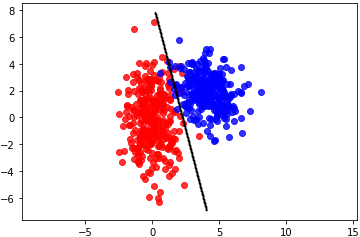
\includegraphics[width=.8\linewidth]{Code/images/42/LDAex}
		\caption{LDA}
	\end{subfigure}%
	\begin{subfigure}{.5\textwidth}
		\centering
		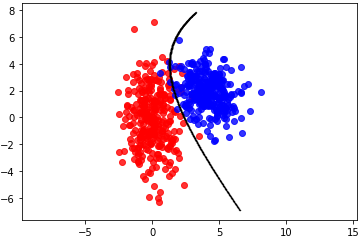
\includegraphics[width=.8\linewidth]{Code/images/42/QDAex}
		\caption{QDA}
	\end{subfigure}
	\caption{Example of LDA and QDA where the decision boundary is shown in black.}
	\label{fig:LQDAex}
\end{figure}
We note that both LDA and QDA are equivalent to the Bayes rule \ref{bayesclass} when the assumptions of normality and homoscedasticity (for the LDA) are satisfied. Indeed, the likelihood ratio $f_1(x)/f_0(x)$ is equal to the Radon-Nikodym derivative of the two induced Gaussian measures in this case.

In practice, none of the parameters $\mu_i,\Sigma_i$ are known. They can be estimated in the usual way by the empirical estimators $\hat{\mu}_i,\hat{\Sigma}_i$. These can then be plugged into either the LDA or QDA rules. 


\section{Classification of functional fragments}
\subsection{Explain the work done by Kraus and Delaigle and Hall on the classification of functional fragments and my work}
\section{A probabilistic approach to classification}
\subsection{Explain the perfect classification phenomenon through the F-H theorem. If I manage to find something, also the classification of fragments.}

\chapter{Numerical experiments}









\bibliography{biblio} 
\bibliographystyle{apalike}



\end{document}